\documentclass{article}[18pt]
\usepackage{../../../../../format}
\lhead{MCS - Discrete Mathematics and Linear Algebra}
\usepackage{amsmath}

\begin{document}
\begin{center}
\underline{\huge Basic Counting and Binomial Coefficients}
\end{center}
\section{Binomial Coefficients}
\subsection{Definition}
The number of r-combinations of a set with n distinct elements (with $r\leqslant n$) is denoted by C(n,r). It is also denoted by:
$$\binom{n}{r}$$
and is called a \textbf{binomial coefficient}\\
\\
"n choose r" refers to counting the number of different subsets of r elements from a set of n elements, so by literally choosing r elements from n elements in all possible ways
\subsection{Example}
\textit{How many National Lottery combinations are there?}
$$\binom{49}{6}=\dfrac{49!}{6!43!}=\dfrac{49\cdot48\cdot47\cdot46\cdot45\cdot44}{1\cdot2\cdot3\cdot4\cdot5\cdot6}=13,938,816$$
\subsection{A simple property of binomial coefficients}
\subsubsection{Proposition}
\textit{For any integers $0\leqslant k\leqslant n$}
$$\binom{n}{k}=\binom{n}{n-k}$$
\subsubsection{Proof}
\begin{itemize}
\item Selecting k objects out of n is the same as leaving out k-n elements
\item LHS counts the number of ways to select k
\item RHS counts the number of ways to leave n-k out
\end{itemize}
\section{Pascal's identity}
\subsection{Theorem}
\textit{Let n and k be positive integers with $n\geqslant k$. Then:}
$$\binom{n+1}{k}=\binom{n}{k-1}+\binom{n}{k}$$
\subsection{Proof}
\subsubsection{Direct Proof}
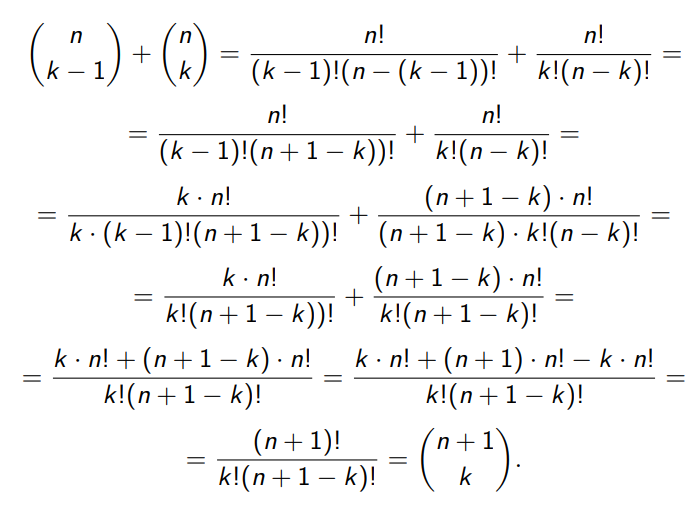
\includegraphics[width=8cm]{pascal_proof.png}
\subsubsection{Combinatorial Proof}
Pascal's Identity:
$$\binom{n+1}{k}=\binom{n}{k-1}+\binom{n}{k}$$
Show that both sides of the identity count the same things in a different way:
\begin{itemize}
\item The left hand side counts all the possible subsets of k elements from a set of n+1 elements

\item Fix one element x. The right hand side counts:
\begin{itemize}
\item All the possible k subsets containing x (we have to choose another k-1 elements from the other n elements) plus,
\item All the possible k subsets not containing x (we still have to choose k elements from the other n elements)
\end{itemize}
\end{itemize}
\section{Pascal's Triangle and Binomial Coefficients}
\begin{center}
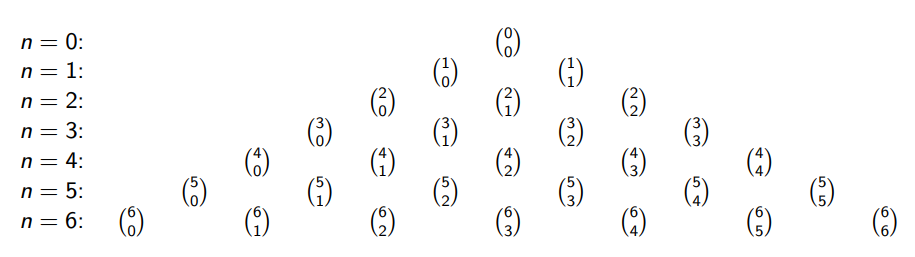
\includegraphics[scale=0.7]{pascal_triangle_1.png}\\
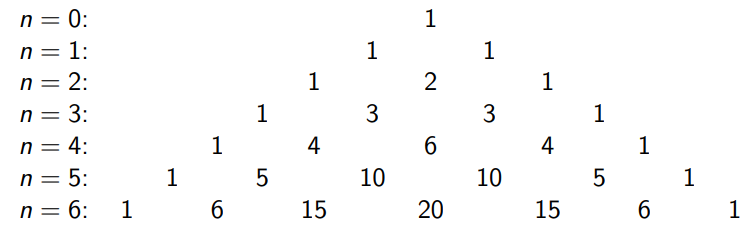
\includegraphics[scale=0.7]{pascal_triangle_2.png}
\end{center}
\section{Binomial Theorem}
\subsection{Theorem}
\textit{Let x and y be variables, and let n be a nonnegative integer. Then}
$$(x+y)^n=\binom{n}{0}x^n+\binom{n}{1}x^{n-1}y+\binom{n}{2}x^{n-2}y^2+...+\binom{n}{n-2}x^2y^{n-2}+\binom{n}{n-1}xy^{n-1}+\binom{n}{n}y^n$$
\subsection{Examples}
$$(x+y)^2=x^2+2xy+y^2$$
$$(x+y)^3=x^3+3x^2y+3xy^2+y^3$$
The coefficients are rows in Pascal's triangle
\subsection{Idea of the proof}
\begin{itemize}
\item In the expansion of $(x+y)^n$ we obtain the value of "n choose k" as the coefficient of the term $x^{n-k}y^{k}$
\item This is because one has to choose a y from k of the n brackets x+y in the expansion; the other n-k are all x
\end{itemize}
\subsection{Examples}
\textit{Prove that}
$$\binom{n}{0}+\binom{n}{1}+\binom{n}{2}+	\binom{n}{3}+...+\binom{n}{n}=2^n$$
Solution: Use the binomial formula with $x=y=1$
\section{Permutations with indistinguishable objects}
\subsection{Theorem}
\textit{The number of different permutations of n objects, of which there are\\
$n_1$ indistinguishable objects of type 1\\
$n_2$ indistinguishable objects of type 2\\
...,\\
$n_k$ indistinguishable objects of type k, is
}
$$\dfrac{n!}{n_1!n_2!...n_k!}$$
As with anagrams
\begin{itemize}
\item There are $C(n,n_1)$ choices to put $n_1$ type 1 objects in n positions
\item Then $C(n-n_1,n_2)$ choices t put $n_2$ type 2 objects in the remaining $n-n_1$ positions, and so on
\end{itemize}
The total number is:
$$C(n,n_1)\cdot C(n-n_1,n_2),...,C(n-n_1-n_2-...n_{k-1}-n_k)=\dfrac{n!}{n_1!n_2!...n_k!}$$
\section{Combinations with Indistinguishable Objects}
\textbf{Multiset} - A set in which each element a has a multiplicity (times they appear) $n_a$\\
\textit{Example: [0,0,1,2,2,2]=[1,0,2,2,0,2] is a multiset of size 6, with $n_0=2$, $n_1=1$, $n_2=3$}
An r-combination of n objects with repetition is a multiset of size r whose elements come from these n objects\\
\\
Using the idea with bars and stars, one can show the following:
\subsection{Theorem}
The number of different r combinations of n objects with repetitions is $C(n+r-1,n-1)=C(n+r-1,r)$

\section{Additional Slides}
\section{Distributing Objects into Boxes}
\textit{How many ways are there to distribute n objects into k boxes?}\\
The answer depends of whether the objects/boxes are distinguishable
\begin{itemize}
\item D objects into D boxes
\begin{itemize}
\item Ex. Dealing 52 cards to 4 people
\end{itemize}

\item inD objects into D Boxes
\begin{itemize}
\item Identical balls into numbered boxes
\end{itemize}

\item D objects into inD Boxes
\begin{itemize}
\item Numbered balls into identical boxes
\end{itemize}

\item inD objects into inD Boxes
\begin{itemize}
\item Identical balls into identical boxes
\end{itemize}

\end{itemize}
\subsection{Objects into D-Boxes}
\textbf{D-Objects into D-Boxes: numbered balls into numbered boxes}\subsubsection{Theorem}
The number of ways to distribute n D-Objects into k D-boxes so that box i receives $n_i$ objects is:
$$\dfrac{n!}{n_1!n_2!,...,n_k!}$$
\textbf{inD objects into D boxes: Identical balls into numbered boxes}
\subsubsection{Theorem}
The number of ways to distribute n inD objects into k D-Boxes is
$$C(n+k-1,k)$$
\subsection{Objects into inD-Boxes}
\textbf{D-Objects into inD-Boxes: n numbered balls into k identical boxes}\\
Same as counting partitions of the balls into $\leqslant$ k parts
\subsubsection{Fact}
A simple closed formula for the number of ways to distribute n D-Objects into k inD-Boxes is\\
NOT KNOWN
\textbf{D-Objects into inD Boxes: n identical balls into k identical boxes}
\subsubsection{Fact}
A simple closed formula for the number of ways to distribute n inD-Objects into k inD boxes is:\\
NOT KNOWN


\end{document}